%!TEX root = main.tex

\chapter{Marketing Mix Modeling}

\begin{chapquote}{John Wanamaker}
	``"La mitad del dinero que me gasto en publicidad es un desperdicio: el problema es que no sé qué mitad es.''
\end{chapquote}

\comment{contextualizar con otras partes del libro, mencionar la motivación y de por que esta este capitulo en el libro.}

\comment{parrafo: agregar resumen del capitulo y los temas que se mencionan}

El modelado de mezcla de marketing, conocido como (\emph{marketing mix modeling} en inglés denotado como MMM) constituye una técnica de modelado destinada a discernir las conexiones entre la inversión en marketing en diversos canales y los logros alcanzados, ya sea en términos de tráfico web, ventas, captación de clientes u otros idicadores clave de rendimiento (\emph{key performance indicator} en inglés denotado como KPI). El enfoque del MMM se basa en el análisis de datos históricos y la aplicación de métodos de regresión para desentrañar la contribución de cada canal en relación con los KPI.

En este capítulo, se expondrán y detallarán los aspectos fundamentales de nuestra metodología en el ámbito del MMM. Se ofrecerá una panorámica del modelo básico empleado, seguido de una descripción minuciosa con el enfoque de aprendizaje automático bayesiano.

\section{Introducción al MMM}

La revolución de los grandes datos de los últimos años se deriva del aumento en la cantidad de datos disponibles, la expansión del poder de cómputo y los avances en los algoritmos de aprendizaje profundo utilizados por los profesionales. A la luz de la forma en que se ha desarrollado el campo, puede parecer que cualquier problema que involucre datos puede resolverse con éxito mediante una aplicación de procesamiento numérico suficiente.

La realidad, sin embargo, es que para una gran clase de problemas, la cantidad de datos disponibles es demasiado pequeña para que las técnicas de aprendizaje profundo sean aplicables. Esta es la categoría en la que cae MMM: los volúmenes de datos sobre gastos de marketing y ventas u otras métricas comerciales relevantes que están disponibles al construir un MMM están lejos de los utilizados en el ámbito de las grandes empresas de big data. Esto es inherente a los problemas de regresión de series temporales, donde el horizonte temporal de los datos disponibles es cercano a los tres años en un caso ideal, es decir, menos de doscientos puntos temporales semanales.

El gran desafío en MMM es extraer la mayor cantidad de inteligencia posible de pequeños conjuntos de datos para brindar una solución que funcione para la mayoría de los anunciantes. Logramos esto mediante el uso de un enfoque bayesiano de MMM, que es diferente en varios aspectos del marco clásico basado en la regresión.


\section{Input Data}

Comenzamos con un conjunto de datos indexados en el tiempo (generalmente ventas) \(\mathcal{D} = \{(t_1, y_1), \dotsc, (t_n, y_n)\}\) y variables explicativas indexadas en el tiempo.

\begin{figure}[h]
	\centering
	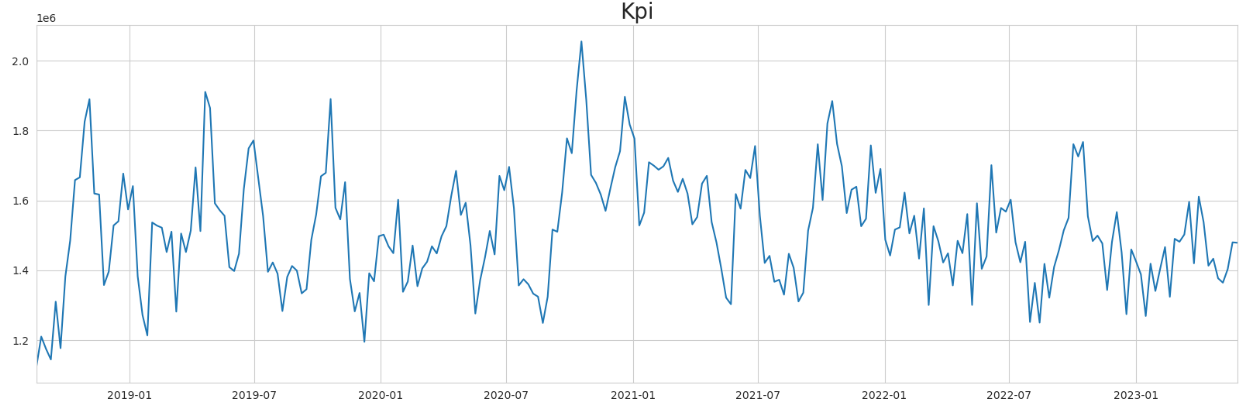
\includegraphics[width=0.9\textwidth]{KPI}
	\caption{Ejemplo de un serie de KPI.}\label{KPI}
\end{figure}

La cantidad mínima de datos necesaria para estimar un modelo de mezcla de marketing es una variable dependiente (generalmente ventas, denotadas por \(y_0, \dotsc y_t\)), y series de inversión para una cantidad de medios, denotadas \(x_0^m, \dotsc, x_t^m\), y \(m \in M\) es el conjunto de medios. Siempre que hablamos de series asumimos que son series temporales, indexadas en el tiempo.


\begin{figure}[h]
	\centering
	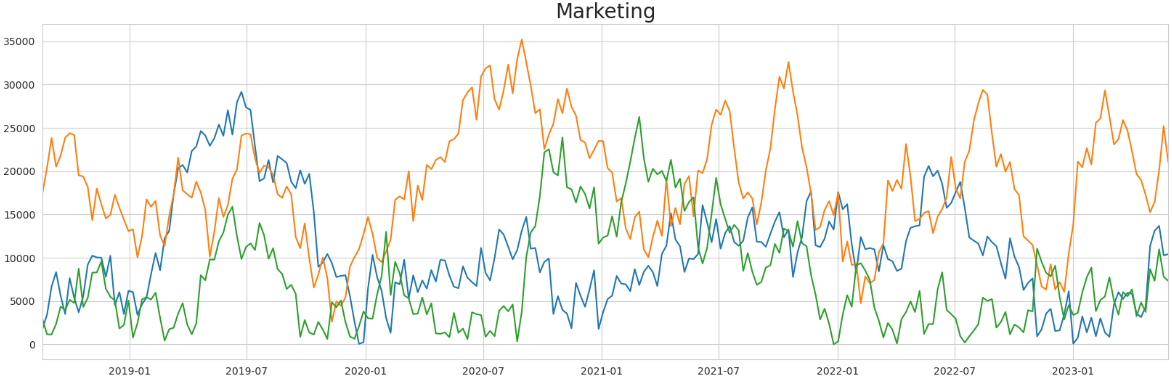
\includegraphics[width=0.9\textwidth]{Marketing}
	\caption{Ejemplo de series de marketing.}\label{Marketing}
\end{figure}

Otros datos opcionales que se pueden considerar son la inversión de la competencia, las inversiones no controlables, el precio, la distribución, las variables macroeconómicas, las fechas especiales, etc. Nuevamente, estas deben ser series de tiempo.

Sin pérdida de generalidad, cada serie se reducirá en el intervalo \([-1, 1]\) para trabajar. Algunas series se reducirán utilizando el cuantil 95 ya que deben ser no negativas (como gasto o ventas), mientras que otras se normalizarán (centradas y normalizadas por la desviación estándar), como precio, distribución u otras.

\subsection{MMM}


Para simplificar, supondremos aquí que la variable objetivo corresponde a las ventas, aunque la estructura básica del modelo se puede aplicar a una variedad de otras métricas comerciales de interés (como visitas a tiendas o un sitio web, oportunidades de ventas o el número de clientes captados de los competidores) con sólo modificaciones menores. Para cada período de tiempo $t$, las ventas ($S_t$) se descomponen como el producto entre un componente de tendencia, compuesta por una componente incremental y una componente base, y una componente de estacionalidad: \medskip
\begin{equation*}
\tikzmark{s} S_t ~~~=~~~ \tikzmark{t} T_t \, \cdot \, F_t \tikzmark{p}.
\begin{tikzpicture}[overlay,remember picture]
\node (S1) [left of = s, node distance = 4.5em, yshift=0.5em]{\footnotesize ventas};
\node (S2) [left of = s, node distance = 0em, yshift=0.25em]{};
\draw[->, in=180, out=350] (S1.east) to (S2.west);
\node (T1) [left of = t, node distance = 4.5em, yshift=1.5em]{\footnotesize tendencia};
\node (T2) [left of = t, node distance = 0em, yshift=0.8em]{};
\draw[->, in=150, out=350] (T1.east) to (T2.west);
\node (P1) [right of = p, node distance = 4.5em, yshift=1.5em]{\footnotesize factor};
\node (P2) [right of = p, node distance = -0.5em, yshift=0.8em]{};
\draw[->, in=45, out=210] (P1.west) to (P2.east);
\end{tikzpicture}
\end{equation*}

La componente de tendencia de las ventas $T_t$ se da a su vez como la suma de dos componentes de ventas incrementales más las ventas bases:\medskip
\begin{equation*}
\tikzmark{t} T_t ~~~=~~~ \tikzmark{im} I^\calM_t ~+~ I^\calC_t \tikzmark{ic} ~+~ B_t \tikzmark{b}.
\begin{tikzpicture}[overlay,remember picture]
\node (E1) [left of = im, node distance = 4.5em, yshift=1.5em]{\footnotesize marketing inc.};
\node (E2) [left of = im, node distance = 0em, yshift=0.8em]{};
\draw[->, in=150, out=350] (E1.east) to (E2.west);
\node (T1) [right of = ic, node distance = 5.5em, yshift=1.3em]{\footnotesize no controlable inc.};
\node (T2) [right of = ic, node distance = 0em, yshift=0.8em]{};
\draw[->, in=25, out=200] (T1.west) to (T2.east);
\node (B1) [right of = b, node distance = 4.5em, yshift=0.5em]{\footnotesize base};
\node (B2) [right of = b, node distance = 0em, yshift=0.25em]{};
\draw[->, in=0, out=180] (B1.west) to (B2.east);
\end{tikzpicture}
\end{equation*}

Los componentes incrementales $I_t = I^\calM_t + I^\calC_t$ modelan ventas que resultan, respectivamente, directamente de acciones de marketing y de acciones no controladas por el cliente. En la versión más básica del modelo, $I^\calM_t$ se modela como una suma sobre las ventas que son atribuibles directamente al gasto en cada uno de los diferentes canales de medios,
\begin{equation}\label{incremental}
\tikzmark{i} I^\calM_t ~~~=~~~ \sum_{m=1}^{\tikzmark{mtot} M} A^{(m)}_t \tikzmark{a}.
\begin{tikzpicture}[overlay,remember picture]
% \node (I1) [left of = i, node distance = 4.5em, yshift=0.6em]{\footnotesize incremental};
% \node (I2) [left of = i, node distance = 0em, yshift=0.25em]{};
% \draw[->, in=180, out=350] (I1.east) to (I2.west);
\node (M1) [left of = mtot, node distance = 9.5em, yshift=0.5em]{\footnotesize número de medios};
\node (M2) [left of = mtot, node distance = 0em, yshift=0.2em]{};
\draw[->, in=185, out=0] (M1.east) to (M2.west);
\node (A1) [right of = a, node distance = 9.5em, yshift=0.85em]{\footnotesize adstock del medio $m$};
\node (A2) [right of = a, node distance = 0em, yshift=0.8em]{};
\draw[->, in=10, out=185] (A1.west) to (A2.east);
\end{tikzpicture}
\end{equation}

El incremental no controlable $I^\calC_t$ se modela de manera similar. La componente de factor $F_t$ tiene un patrón cíclico y debe considerarse como un factor multiplicativo que oscila alrededor de $1$ para representar los diversos efectos estacionales a lo largo de múltiples periodicidades (semanales, mensuales, anuales) que se estiman por separado; este componente también tiene en cuenta campañas o eventos especiales únicos. Toda esta notación nos permite escribir nuestro modelo de una manera más clara como
\[f_t = (I_t + B_t) (1 + V_t).\]

Cada término tiene un significado distinto: en el momento \(t\), la componente incremental \(I_t\) representa el efecto de marketing (y otros efectos aditivos), la componente base \(B_t\) representa las ventas no directamente atribuibles a \( I_t\), y \(V_t\) representa las variaciones dadas por efectos temporales y otros efectos multiplicativos. Aclaramos que \(I_t\) y \(V_t\) son paramétricos y dependen de los datos de entrada (gastos de marketing, variables económicas, estacionalidades, precio, distribución, etc.), mientras que \(B_t\) no es paramétrico.

Ahora definimos varias cantidades de interés para el modelo:
\begin{itemize}
	\item La \emph{variación} es simplemente \(V_t\).
	\item El \emph{factor} se define como \(F_t = 1+V_t\).
	\item La \emph{tendencia} se define como \(T_t = I_t + B_t = \frac{f_t}{1+V_t}\).
	\item El término \emph{aditivo} se define como \(D_t = f_t - T_t = T_t V_t\).
	\item La componente \emph{explicado} se define como \(E_t = I_t (1 + V_t)\).
	\item La componente \emph{no explicado} se define como \(U_t = B_t (1 + V_t)\).
\end{itemize}

A continuación se expone un diagrama de un MMM básico.
\begin{figure}[h]
	\centering
	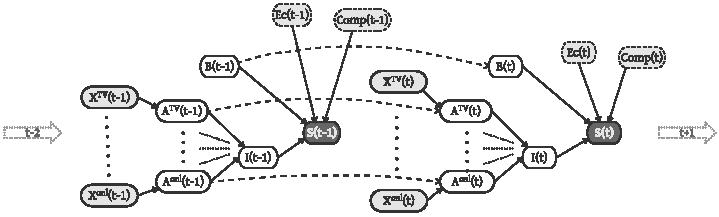
\includegraphics[width=\textwidth]{MMM.pdf}
	\caption{El MMM básico. Por ejemplo, las variables de stock publicitario $A^{\rm TV}(t),\dotsc,A^{\rm online}(t)$ dependen del nivel de inversión en los medios asociados en el período dado, $X^ {\rm TV}(t),\dotsc,X^{\rm online}(t)$, y en los niveles de acciones publicitarias del período anterior. Los detalles de esta dependencia se especifican como una propiedad del nodo adstock. En esta red también añadimos dependencia de las ventas $S\hspace{-0.15ex}(t)$ de un conjunto de variables económicas y de información sobre la competencia, ${\rm Ec}(t)$ y ${\rm Comp}(t)$.}\label{MMM-DBN}
\end{figure}

\subsection{Adstocks}
\label{subsec:adstocks}

\textit{Adstock} aquí se refiere al efecto agregado (medido como ventas) de los esfuerzos de marketing en los períodos actuales y pasados en un canal de medios determinado (en una versión más general del modelo, los anuncios de diferentes puntos de contacto de medios se pueden combinar en cualquier otra forma para modelar los efectos multiplicadores no lineales resultantes de acciones en diferentes medios). Al modelar la evolución del stock de anuncios publicitarios, se deben considerar tres aspectos: los efectos retardados o rezagados de las acciones publicitarias, la disminución de estos efectos a lo largo del tiempo y el efecto de saturación al que está sujeto el gasto en marketing. La dinámica básica de las acciones publicitarias en nuestro modelo implica, por lo tanto, una combinación entre los efectos de la publicidad en el período actual y en el pasado.


El adstock es, en palabras simples, el efecto que ha tenido una inversión a lo largo del tiempo. Construimos este efecto de la siguiente manera: primero definimos una función \(H\) en forma de S, llamada \textit{saturación}, usando dos parámetros \(u \in (0,1)\) y \(b > 0 \) (el punto de semisaturación y un parámetro de forma), de la siguiente manera:
\[ H_{ u,b }(x) = \frac{ x^b }{ u^b + x^b }. \]

Si \(x\) es un valor de gasto, \(H(x)\) modela la saturación de dicho gasto. Claramente tenemos que \( H(x) \in [0,1) \) y \(H(x) \to 1\) como \(x \to \infty\). \(u\) se llama semisaturación porque \(H(u) = 1/2\) (recuerde que la inversión se reduce, por lo que para recuperar \(u\) en la escala original simplemente multiplicamos \(u\) por la escala de esa serie).

\begin{figure}
	\centering
	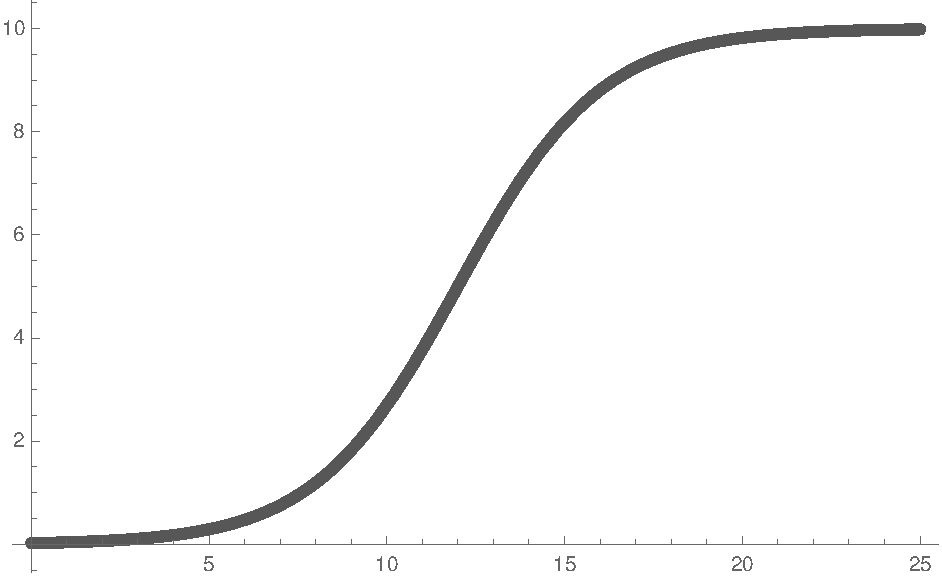
\includegraphics[width=0.52\textwidth]{logistic.pdf}
	\caption{Función sigmoidea típica \(H_m\). Depende de un conjunto de parámetros que controlan las principales características de su forma: el nivel de saturación (aquí alrededor de 10), el nivel de inversión en el que se alcanza la saturación (aquí alrededor de 22) y el punto donde comienzan los rendimientos decrecientes (es decir, donde la curva cambia de convexa a cóncava, aquí alrededor de 12)}
	\label{logística}
\end{figure}

Agregamos otro parámetro \(c\), el carry-cap, para modelar el efecto actual de un gasto a la vez. Entonces, en el momento \(s\) y la inversión \(x_s\), \(cH(x_s)\) modela el impacto en el momento \(s\) de la inversión saturada. Aunque técnicamente tenemos que \(c > 0\), a continuación especificamos que (y por qué) \(c \in (0,1)\).

Para modelar el efecto que ha tenido el gasto en el tiempo consideramos un retraso \(p\) en el tiempo (perdón por la redundancia) que afecta a los términos \(cH(x_s)\) en el tiempo. En detalle, \(p\) es una distribución binomial negativa\footnote{Esta variable aleatoria modela la probabilidad de obtener \(k\) éxitos al lanzar una moneda con probabilidad \(d\) de éxito dado que \(r\) ( no aleatorios) deben ocurrir fallas.}, uno versátil que nos permite modelar muchas formas de retraso. Dicha distribución está definida por dos parámetros \(d \in [0,1]\), \(r_l \in \naturals\), llamados decay y r-lag, que son la probabilidad de la moneda y la moda de la binomial negativa . La media de \(p\) viene dada por \(r = (1 - d) r_l / d + 1 \) y la distribución es:
\[ p(s) = \frac{ \Gamma(s + r) }{ s! \Gamma(r) } (1 - d)^{r} d^s. \]
Un valor más bajo de \(d\) implicará un retraso más rápido, ya que una menor probabilidad de éxito implicará acumular los fallos corregidos (aquí \(r\)) rápidamente. $r_l$ es la semana/mes donde un pulso de inversión alcanza su efecto máximo.


Juntando todo esto, para una serie de gastos \(x_0, \dotsc, x_t\) la función adstock para un medio \(m\) es una convolución en el tiempo entre la curva \(cH\) y el retraso \(p \):
\[ A(x_0^m, \dotsc, x_t^m) = \sum_{s=0}^t p(t-s) c H(x_s^m). \]
Un pequeño detalle a tener en cuenta es este: los datos tienen un tiempo de inicio, y no es posible tener datos antes de ese tiempo. Incluimos entonces otro término, un ``gasto en tiempo pasado'', denotado \(x_{-1}^m\) y denominado init-control, que pretende representar todo el gasto realizado antes de la primera vez de los datos. Este control de inicio también está saturado y complicado con \(p\). Por lo tanto, la función adstock se modifica para
\[ A(x_0^m, \dotsc, x_t^m) = \sum_{s=0}^t p(t-s) cH(x_s^m) + [1 - F_p(t+1)] cH(x_{- 1}^m), \]
donde \(F_p\) es la distribución acumulada de \(p\). Para una serie de gasto \((x_0^m, \dotsc, x_t^m)\) los parámetros \(c, u, b, d, r, x_{-1}\) deben ser entrenados para dicho \(m\).

La curva de descomposición $p_m$ se estima por separado para cada medio y modela la tasa a la que el efecto de una acción de marketing determinada en ese medio decae con el tiempo. $H_m$, por otro lado, es una función de forma sigmoidea que modela el efecto de saturación del gasto en un medio dado (ver Figura \ref{logística}). Esta curva de saturación se estima por separado para cada medio.

Dado que todas las inversiones deben modelarse como acciones publicitarias, también incluimos un parámetro de escala \(\alpha\) para entrenar, que modela el impacto de todas las acciones publicitarias de la siguiente manera:
\[ I_t^M = \alpha \sum_{m \in M} A(x_0^m, \dotsc, x_t^m). \]
Tenga en cuenta que \(\alpha\) multiplica todos los carry-caps, por lo que normalizamos todos los carry-caps a \([0,1]\) (y suman 1). Por lo general, se agrega una serie de stock publicitario (es decir, como una suma) al incremental. El efecto incremental es la suma de todos los incrementales, es decir \( I_t = I_t^M + I_t^{M'} + I_t^{M''} + \dotsb, \) donde los \(M\) posteriores son diferentes conjuntos de datos.


\subsection{Saturaciones}

Algunas series, como la económica, la de precios, la de distribución o las de valores atípicos, se pueden modelar mediante saturaciones. Actualmente consideramos cuatro efectos de saturación donde, independientemente del método, se debe entrenar un peso \(w\) y una escala \(\alpha\).
\begin{enumerate}
	\item Saturación por defecto: \(E(z_t) = \alpha \tanh(w z_t)\),
	\item Saturación lineal: \(E(z_t) = \alpha w z_t\),
	\item ``Uno más'' saturación: \(E(z_t) = 1 + \alpha \tanh(w z_t)\),
	\item ``Uno más'' saturación lineal: \(E(z_t) = 1 + \alpha w z_t\),
\end{enumerate}
Los dos primeros se suelen sumar al incremental. Los dos últimos se multiplican por el factor.

\subsection{Estacionalidad}

Un efecto particular que consideramos (multiplicado al factor actual) es el efecto estacional. Intentamos estimar una suma de senos y cosenos donde los periodos son las divisiones habituales de un año: un año entero, un semestre, un cuatrimestre, un trimestre, un bimestre y un mes. El efecto se define como
\[ Es(t) = 1 + \alpha \sum_{p\in P} c^1_p \sin\left(\frac{2\pi t}{p \varepsilon}\right) + c^2_p \cos \left(\frac{2\pi t}{p \varepsilon}\right),\]
donde \(P\) es el conjunto de periodos y \(\varepsilon \sim 1\) es un pequeño jitter en el caso semanal, pero igual a \(1\) en el caso mensual. Se deben entrenar los parámetros \(\varepsilon\) y \(c^1_p, c^2_p\), para todos los períodos.

\section{MMM as TGP}

Nuestro modelo es una regresión de la forma de un Proceso Gaussiano de Transporte (TGP) denotado \(f \sim \mathcal{TGP}(h, k)\), donde \(h\) es un transporte marginal y \(k\) un kernel de covarianza. A continuación explicamos cómo se eligen estas funciones \(h\) y \(k\) para dar forma al modelo final.

Observamos que dado que este es un problema de regresión, nuestro objetivo es encontrar el mejor predictor \(f\) tal que \(f\) esté cerca de los puntos de datos \(y\).

\subsection{Base}

Nuestra descripción hasta ahora ha sido puramente determinista, pero en realidad también debemos considerar la incertidumbre sobre lo que no podemos observar ni medir. Para ello añadimos dos componentes estocásticos diferentes. El primero es un vector de componentes base que pretende representar ventas base aleatorias.

El kernel de covarianza \(k\) determina la componente no paramétrico del modelo, que llamamos base. Este transporte de covarianza con el ruido viene dado por
\begin{align*}
k(s, t)	&= (1-\sigma) r(s, t) + \sigma \delta(s, t),\\
r(s, t)	&= \mathrm{SE}_{\ell_l}(s, t) \; \mathrm{SE}_{\ell_s}(s, t),\\
\mathrm{SE}_{\ell}(s, t) &= \exp\left( -\left(\frac{s-t}{100 \; \ell}\right)^2 \right),
\end{align*}
donde \(\sigma \in (0, 1)\) es la escala de ruido, \(\ell_l \in (0, 1)\) y \(\ell_s \in (0, 1)\) son largas y escalas de longitud corta, y \(\delta\) es el delta de Kronecker. Especificamos que \(\ell_s < \ell_l\).

Después de esto, consideramos el transporte marginal \( h_R(t, x) = \alpha \relu(2 + x) \). La razón para hacer esto es ``mover'' el proceso gaussiano generado por \(k\) lejos de \(0\), dejando solo alrededor de \(2\%\) de la masa debajo de \(0\). El \(\relu\) luego concentra este \(2\%\) de masa en \(0\). Esto da como resultado un TGP con distribuciones marginales gaussianas rectificadas (de ahí el subíndice \(R\)) y, por ahora, el TGP tiene la forma \( f \sim \mathcal{TGP}(h_R, k) \). Se deben entrenar los hiperparámetros $\sigma$, $\ell_l$, $\ell_s$ y $\alpha$.

\subsection{Noise}
Tenga en cuenta que el transporte de covarianza dado por \(k\) tiene ruido, dado por el delta de Kronecker. Podemos hacer la distinción entre un modelo ruidoso y uno silencioso, y simplemente denotar la predicción ruidosa con un superíndice como
\[f^{\mathrm{(n)}}_t = (I_t + B^{\mathrm{(n)}}_t) (1 + V_t).\]
Con esto, la componente de ruido es \(N_t = f_t^{\mathrm{(n)}} - f_t = (B^{\mathrm{(n)}}_t - B_t) (1 + V_t)\). En aras de la exhaustividad también podemos definir
\begin{itemize}
	\item The \emph{base ruidoso} as \(B^{\mathrm{(n)}}_t = B_t + \frac{N_t}{1 + V_t}\).
	\item The \emph{inexplicable ruidoso} as \(U^{\mathrm{(n)}}_t = U_t + N_t = B^{\mathrm{(n)}}_t (1 + V_t)\).
\end{itemize}
Finalmente, dado que \(y_t\) denota los datos observados (la variable a explicar), podemos definir la componente residual como \(R_t = f^{\mathrm{(o)}}_t - f_t = y_t - f_t\), donde el superíndice significa \emph{observado}. Especificamos que \( f^{\mathrm{(o)}}_t \stackrel{\mathrm{d}}{=} f^{\mathrm{(n)}}_t \), es decir, la predicción observada y la predicción ruidosa comparten la misma ley de probabilidad, pero es la posterior de la predicción observada la que coincide con los datos en sus tiempos asociados.

Todas las definiciones anteriores nos dan buenas formas diferentes de escribir y hablar sobre el modelo, como
\begin{align*}
f_t					&= (I_t + B_t) (1 + V_t) = T_t + A_t = E_t + U_t,\\
f_t^{\mathrm{(n)}}	&= (I_t + B^\mathrm{(n)}_t) (1 + V_t) = E_t + U_t + N_t,
\end{align*}
es decir, ``la predicción es tendencia más aditivo, pero también es explicado más no explicado''.

\subsection{Incremental}

El segundo y principal componente de nuestro modelo se llama incremental, una componente paramétrica que modela todos los efectos directos sobre la variable dependiente. Dadas algunas variables explicativas indexadas en el tiempo \(S_1, \dotsc, S_n\), la componente incremental viene dado por una función positiva \(I(t, S_1, \dotsc, S_n)\), con el transporte marginal asociado dado por \(h_I(t, x) = I_t + x\), donde \(I_t\) es el incremental en el tiempo \(t\).

Con esto, por ahora el modelo sigue la relación \(f \sim \mathcal{TGP}(h_I \circ h_R, k)\) y se cumple que en el tiempo \(t\) \(f_t = I_t + B_t\), donde \(B \sim \mathcal{TGP}(h_R, k)\) es la componente base.

\subsection{Factor}

Mientras que los componentes incremental y base intentan especificar una tendencia general al modelo, la siguiente componente, el factor, apunta a modelar variaciones alrededor de esta tendencia. Dadas algunas variables explicativas indexadas en el tiempo \(P_1, \dotsc, P_m\), la componente del factor viene dado por una función positiva alrededor de \(1\), específicamente, \(F(t, P_1, \dotsc, P_m) = 1 + V(t, P_1, \dotsc, P_m)\), con \(V\) una función alrededor de \(0\).

El respectivo transporte marginal está dado por \(h_F(t, x) = F_t x\), donde \(F_t\) es el factor en el tiempo \(t\). Por lo tanto, el modelo final sigue que \(f \sim \mathcal{TGP}(h_F \circ h_I \circ h_R, k)\) y satisface que en el tiempo \(t\), \(f_t = (I_t + B_t) F_t\), donde \(B \sim \mathcal{TGP}(h_R, k)\) es la componente base.

\section{Model training}

Entrenamos el modelo utilizando modelos gráficos probabilísticos y, en particular, una red bayesiana dinámica. No entraremos en el detalle de los modelos gráficos, pero hay que señalar que uno de los componentes centrales es su naturaleza bayesiana. Esto nos permite especificar información a priori sobre los hiperparámetros del modelo de forma natural, y eso proporciona un mecanismo para factorizar la información del modelo que no se puede capturar directamente de los datos (generalmente limitados). Este método nos permite utilizar fácilmente una amplia familia de priores multidimensionales. Si denotamos por \(\theta\) el conjunto de parámetros a entrenar y \(\calD\) el conjunto de datos, entonces
\begin{equation}
\label{eq:posterior}
\tikzmark{post}\prob(\theta \mid \calD) ~=~ \frac{\tikzmark{lik} \prob(\calD \mid \theta) \prob(\theta) \tikzmark{pri}}{\int \prob(\calD, \theta) \dd \theta. \tikzmark{marg}} 
\begin{tikzpicture}[overlay, remember picture]
\node (Po1) [left of = post, node distance = 5.5em, yshift=0.6em]{\footnotesize posterior};
\node (Po2) [left of = post, node distance = 0em, yshift=0.2em]{};
\draw [->, in=180, out=350] (Po1.east) to (Po2.west);
\node (Lik1) [left of = lik, node distance = 5.5 em, yshift=1em]{\footnotesize verosimilitud};
\node (Lik2) [left of = lik, node distance = -0.1em, yshift=0.3em]{};
\draw[->, in=180, out=340] (Lik1.east) to (Lik2.west);
\node (Pri1) [right of = pri, node distance = 5.5 em, yshift=1em]{\footnotesize prior};
\node (Pri2) [right of = pri, node distance = -0.1em, yshift=0.3em]{};
\draw[->, in=25, out=215] (Pri1.west) to (Pri2.east);
\node (Mar1) [right of = marg, node distance = 8.5 em, yshift=-0.6em]{\footnotesize evidencia \( \prob(\calD) \)};
\node (Mar2) [right of = marg, node distance = -0.1em, yshift=0.3em]{};
\draw[->, in=-25, out=160] (Mar1.west) to (Mar2.east);
\end{tikzpicture}
\end{equation}


Un enfoque estándar para encontrar los parámetros es maximizar la parte posterior de este modelo. Aplicando logaritmo a ambos lados e ignorando el término de evidencia (ya que es una constante en \(\theta\)), tenemos que
\[ \log (\prob(\theta \mid \calD)) \propto \log(\prob( \calD \mid \theta )) + \log(\prob(\theta)). \]
El lado derecho es el log-posterior (logp) (no normalizado), la función objetivo a maximizar. El primer término es el log-verosimilitud, y el segundo es el log-prior. Dado que maximizar es lo mismo que minimizar la función negativa, minimizamos el logaritmo posterior negativo.

Aplicando la regla de la cadena y el teorema del cambio de variables, especificamos la fórmula final, introduciendo la siguiente notación: sean \(\mathbf{t}\) y \(\mathbf{y}\) los puntos de datos en \(\mathcal{D}\) como vectores ; sea \(g_\phi = h_\phi^{-1}\) la inversa de un transporte, para cada símbolo \(\phi \in \{R, I, F\}\); sea \(\mathbf{x} = g_R \circ g_I \circ g_F(\mathbf{t}, \mathbf{y})\) la composición de los inversos en orden inverso; y sea \(\Sigma_{\mathbf{xx}}\) la matriz de covarianza dada por el kernel \(k\). Entonces la log-verosimilitud es
\begin{align*}
-\log(\prob(\calD \mid \theta)) =	& \underbrace{\frac{n}{2} \log(2\pi)}_{\text{término constante}} + \underbrace{\frac{1}{2}\mathbf{x}^\top \Sigma_{\mathbf{xx}} \mathbf{x}}_{\text{término de ajuste}} + \underbrace{\frac{1}{2} \log |\Sigma_{\mathbf{xx}}|}_{\substack{\text{término de}\\ \text{complejidad del kernel}}}\\
& - \underbrace{ \log|\nabla g_R (\mathbf{t}, g_I \circ g_F (\mathbf{t}, \mathbf{y}))| - \log|\nabla g_I (\mathbf{t}, g_F (\mathbf{t}, \mathbf{y}))| - \log|\nabla g_F (\mathbf{t}, \mathbf{y})|}_{\substack{\text{término de complejidad del transporte}}}.
\end{align*}


\subsection{Priors}

Dado que nuestro enfoque para estimar los parámetros es bayesiano, debemos especificar los priores de los parámetros. Para cada parámetro \( \theta \), cualquiera de los enumerados anteriormente, su anterior es una versión especial de la distribución Beta, llamada ``Ubicación Beta'', porque es lo suficientemente flexible para modelar muchas formas de distribución. Esta distribución está definida por cuatro parámetros: un límite inferior \(l\) y un límite superior \(u\) que definen el soporte \( [l, u] \), y dos parámetros de forma \(\alpha, \beta > 0\). Denotamos esto por \( \theta \sim \Betaloc(l, u, \alpha, \beta)\).

Algunas notas sobre esta distribución. Primero, \(\alpha\) y \(\beta\) pueden interpretarse como parámetros de penalización, donde un alto \(\alpha\) hace que la distribución tenga una masa baja en su lado izquierdo (cerca de \( l\)); ídem con \(\beta\) y \(u\) en el lado derecho. También tenemos que los cuatro parámetros caracterizan completamente la media y la moda de la distribución por
\begin{align*}
\mu	&= l + \frac{\alpha}{\alpha + \beta} (u-l),	& \nu	&= l + \nu_{\Beta(\alpha, \beta)} (u-l),
\end{align*}
where the mode of \(\Beta\) is
	\[ \nu_{\Beta(\alpha, \beta)} =
\left\{ \begin{matrix*}[l]
\frac{\alpha - 1}{\alpha + \beta - 2}	& \alpha > 1, \beta > 1;	& 0	& \alpha \leq 1, \beta > 1;\\
\text{any value in } (0,1)				& \alpha = 1, \beta = 1;	& 1	& \alpha > 1, \beta \leq 1;\\
\{0,1\}									& \alpha < 1, \beta < 1.	& 	& \\
\end{matrix*} \right.
\]
La \(\Betaloc\) nos permite usar cualquier par de los cuatro parámetros \(\{\alpha, \beta, \mu, \nu\}\) para caracterizar completamente los otros dos. Esto es útil en situaciones donde se necesita una interpretación simple, en lugar de encontrar por ensayo y error un conjunto adecuado de parámetros.

\subsection{Adam: a Stochastic Gradient Descent technique}

Uno de los algoritmos clave utilizados para optimizar la probabilidad de registro son los métodos de descenso de gradiente estocástico (SGD). Estos algoritmos funcionan de manera muy similar a un método de  gradiente pero, en lugar de considerar todos los datos disponibles, eligen un subconjunto aleatorio de ellos en cada iteración. Recuerde que un algoritmo Vanilla SGD minimiza una función \(L\) (en nuestro caso, la probabilidad logarítmica negativa) sobre los parámetros \(\mathbf{\theta}\) usando una tasa de aprendizaje \(\alpha\) iterando como
\[ \theta_{t+1} \gets \theta_t - \alpha \frac{\partial L}{\partial \theta_t}, \]
El método particular utilizado es Adam (estimación de momento adaptativo), una técnica SGD que actualiza tanto la componente de gradiente como la tasa de aprendizaje. Primero calculamos estimaciones del primer momento (la media) y el segundo momento (varianza no centrada) de los gradientes, utilizando dos tasas de disminución:
\begin{align*}
m_t	&= \beta_1 m_{t-1} + (1-\beta_1) \frac{\partial L}{\partial \theta_t},	& v_t	&= \beta_2 v_{t-1} + (1-\beta_2) \left[\frac{\partial L}{\partial \theta_t}\right]^2,
\end{align*}
donde el cuadrado es por coordenada, y \(m_0 = v_0 = \mathbf{0}\). Para evitar el sesgo hacia \(\mathbf{0}\) corregimos los términos:
\begin{align*}
\hat{m}_t	&= \frac{m_t}{1 - \beta_1^t},	& \hat{v}_t	&= \frac{v_t}{1 - \beta_2^t}.
\end{align*}
Tenga en cuenta que las tasas de decaimiento están elevadas a \(t\). Con estos términos calculamos el siguiente paso:
\[ \theta_{t+1} \gets \theta_t - \frac{\alpha}{\sqrt{\hat{v}_t} + \varepsilon}\hat{m}_t, \]
donde la raíz se toma por coordenada (por lo que la tasa de aprendizaje también se modifica por coordenada)

Una de las razones para usar SGD con datos aleatorios es que el algoritmo evita mínimos locales falsos y el muestreo permite explorar el espacio alrededor de los modos de los parámetros.

\subsection{Markov Chain Monte Carlo (MCMC)}

El segundo algoritmo clave son los métodos MCMC para muestrear estas distribuciones posteriores. En resumen, el principal objetivo de los algoritmos MCMC es obtener muestras de la densidad posterior en la ecuación (\ref{eq:posterior}) cuando las distribuciones anterior y de probabilidad son algo fáciles (aunque no rápidas) de calcular. La evidencia \(\prob(\calD)\) se puede ignorar con seguridad porque las cantidades de intereses son razones y la constante no depende de los valores de los parámetros (por lo tanto, se puede cancelar). Esta característica es importante ya que \(\prob(\calD)\) puede ser difícil de calcular. MCMC es un procedimiento para generar un paseo aleatorio sobre el espacio de los parámetros que, con el tiempo, produce un conjunto representativo de muestras de la distribución. Cada paso de la cadena de Markov \( X(t_i) = \theta_i \) depende únicamente del paso anterior.

En su representación más abstracta, dada una posición \(X(t)\) de la cadena, muestreamos una posición propuesta \(X^*\) a partir de una probabilidad de transición \(\probQ(\cdot \mid X(t))\) y aceptar esta propuesta con probabilidad
\[ \min \left\{ 1, \frac{\prob(X^* \mid \calD)}{\prob(X(t) \mid \calD)} \frac{\probQ(X(t) \mid X^* )}{\probQ(X^* \mid X(t))} \right\}. \]
Si se acepta la propuesta, entonces \(X(t+1) \gets X^*\). De lo contrario, \(X(t+1) \gets X(t)\).

El método de maestro de ceremonias (\emph{emcee} en inglés) involucra la evolución simultánea de un conjunto de \(K\) cadenas \( C = \{X_k\}_{k=1}^K \) en paralelo, y la propuesta de actualizar una de estas cadenas \( X_k \) depende de la posición de las otras cadenas \( C_{[k]}(t) = \{X_j(t)\}_{j\neq k} \). Para actualizar la posición de una cadena \(X_k\) muestreamos aleatoriamente otra cadena \( X_j \) de \( C_{[k]}(t) \) y la posición propuesta es \( X_k(t + 1)\) obtiene \(Y = X_j(t) + Z ( X_k(t) - X_j(t) )\), donde \(Z\) es una variable aleatoria muestreada de una distribución \(g\) que sigue la regla
\[ g(z) \propto
\begin{cases}
\frac{1}{\sqrt{z}}	& \text{if } z \in [1/a, a],\\
0					& \text{otherwise,}
\end{cases}
\]
y el valor de \(a\) se puede modificar (normalmente \( a = 2 \)). La propuesta es aceptada con probabilidad
\[ q = \min \left\{ 1, Z^{N-1} \frac{ \prob(Y) }{ \prob(X_k(t+1)) } \right\}, \]
y \(X_k(t+1) \gets Y\). Si rechaza, \( X_k(t+1) \gets X_k(t) \).

\section{Escenarios}

Una vez que se estima el modelo y se generan los informes, el siguiente paso consiste en emplear el modelo para crear recomendaciones presupuestarias procesables con el objetivo de mejorar las métricas o disminuir el gasto. Nuestro marco de optimización nos permite dar respuestas en una amplia variedad de escenarios. Los dos básicos corresponden a maximizar las ventas y minimizar el gasto necesario para lograr un determinado nivel de ventas, pero hay muchas personalizaciones disponibles, incluida la optimización de acciones publicitarias ponderadas si es necesario tener en cuenta diferentes tasas de conversión, la optimización en un período de tiempo completo o dentro de cada semana, considerando escenarios donde los presupuestos varían en porcentajes fijos, optimizando solo algunos canales de medios y considerando el gasto mensual/trimestral. Las modernas técnicas de optimización y la potencia computacional lograda mediante el uso de GPU nos permiten ejecutar muchos escenarios de optimización en poco tiempo.

Los escenarios en los que nos centramos se pueden dividir en dos categorías principales. Los escenarios hipotéticos implican optimizar la inversión en canales de medios en el pasado, cuando los datos están disponibles. Estos escenarios permiten a los especialistas en marketing comprender cómo podrían haber gastado su presupuesto de manera diferente para obtener mejores resultados. Los escenarios prospectivos, por otro lado, tienen como objetivo optimizar los presupuestos en el futuro, utilizando el modelo para predecir ventas u otras métricas en función de la inversión en diferentes canales.

\section{Marketing Mix}
\label{sec:optimizing}

Una vez que el modelo está entrenado y cargado, se desean hacer dos cosas: una calculadora de planes y un optimizador de planes. A continuación explicamos estas dos funciones, pero antes debemos aclarar un punto importante previo a estos dos ejercicios.

El efecto no paramétrico (la base) se ``congela'' antes que nada, porque las ventas base no pueden cambiar bajo ninguna circunstancia, y deben tener siempre el mismo valor después del entrenamiento. En términos complicados, cualquier ejercicio (calculadora de planes u optimizador de planes) implicará una modificación de algunos componentes del modelo, ya sea en el factor o en el incremental, y ese cambio modificará, en términos matemáticos, los transportes marginales \(h_F\) y \(h_I\). Por lo tanto, los datos \(h_I^{-1} \circ h_F^{-1}(y_t)\) que observa el proceso gaussiano cambian. Congelar la componente base nos permite a nosotros y al cliente comparar ejercicios y predecir ventas que de otro modo no serían posibles, ya que la base se ajustaría a los datos observados.

\subsection{Calculadora de planes}

Esta característica le permite al cliente evaluar montos de inversión en el modelo, como si fuera una función. Las entradas de esta función son el gasto mensual, uno para cada medio, y las modificaciones de las variables externas (es decir, cualquier variable que no sea de marketing controlada directamente por el cliente). Como salida obtenemos las atribuciones (adstocks) para ese marketing mix, ventas previstas y análisis más específicos.

\subsection{Optimizador de planes}

Esta característica le permite al cliente ejecutar escenarios de optimización con restricciones, con el objetivo de recomendar una combinación óptima de medios. Las entradas de esta característica son un lapso de tiempo \(T\), un presupuesto \(b\) a gastar, modificaciones de variables externas y restricciones del tipo
\[ l_m \leq \sum_{t \in T} x_t^m \leq u_m, \]
donde la variable \(x_t^m\) es la inversión en medios \(m\) en el momento (semana/mes) \(t\), y \(l_m\), \(u_m\) son dos límites. Permitimos los siguientes valores: \(l_m \geq 0\); \(u_m\) puede ser igual a \(\infty\) (es decir, sin límite superior); y, cuando \(u_m < \infty\), entonces \(l_m \leq u_m\), por lo que permitimos restricciones de desigualdad e igualdad.

\subsection{Problema de optimización}

Además de las restricciones dadas anteriormente, otra restricción que debe cumplirse es que el presupuesto debe distribuirse a lo largo del tiempo y los medios:
\[ \sum_{m \in M} \sum_{t \in T} x_t^m = b. \]

La restricción final, con respecto a la naturaleza de las variables, es un poco más complicada. Para cada medio tenemos un número llamado \emph{gasto mínimo semanal} \(r_m\), y como su nombre lo dice, invertir en una semana no puede ser menor que \emph{excepto cuando esa inversión es igual a} \(0 \). Entonces, técnicamente, tenemos que \(x_t^m \in \{0\} \cup [r_m, \infty)\).

La función objetivo de este problema de optimización (teórico) es la componente explicada, es decir,
\begin{equation}
\label{eq:strategy}
g(x) = \mean \left[\sum_{t \in T} I_t (1 + V_t)\right],
\end{equation}
donde la expectativa se toma sobre todos los modelos (es decir, el \emph{model average}), considerando que los parámetros que no son de marketing se muestrean solo una vez y se fijan. 